\documentclass{article}
\usepackage[utf8]{inputenc}
\usepackage{graphicx}
\usepackage{amsmath}
\usepackage{gensymb}
\usepackage{titling}
\usepackage{float}

\title{Homework Set 7 - PHYS 728 Radio Astronomy}
\author{Matthew Cooper}
\date{April 2nd, 2019}
\begin{document}
\begin{titlingpage}
    \maketitle
    \begin{abstract}
	This is the report on my methodology for determining $\triangle$Bx, $\triangle$By, and 		$\triangle$Bz from two datasets which were given.  The results of this are that $		 	\triangle$Bx = -.155 m, $\triangle$By = -.044 m, and $\triangle$Bz = -1.565 m, 			 	respectively.  The theory subtracted data is plotted below.
    \end{abstract}
	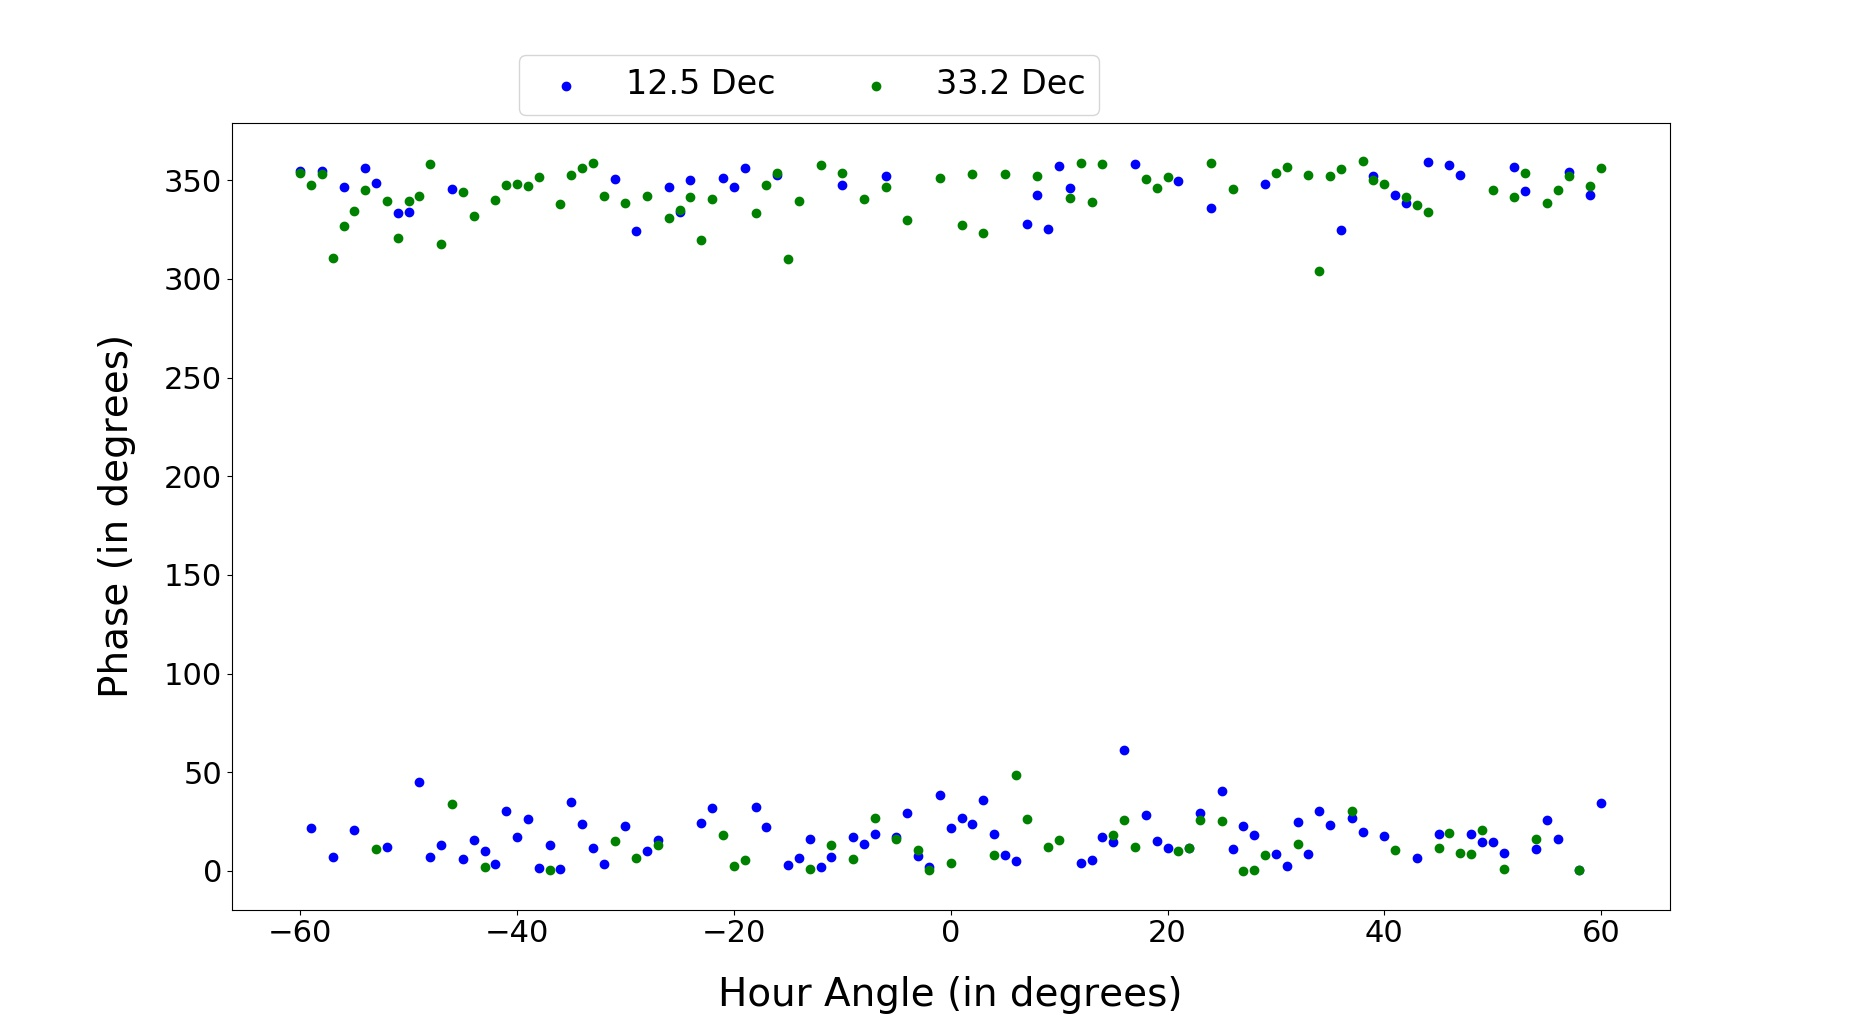
\includegraphics[scale=.25]{/home/matthew/Main/RadioAstronomy/Homework7/DataNoTheory.jpeg}


\end{titlingpage}

\textbf{Problem 7.1}:  The figure below displays the phase at 5 GHz as a function of hour angle (from -60$\degree$ to 60$\degree$) for two different sources, one at 12.5$\degree$ declination and one at 33.2$\degree$ declination. The phases were measured with a baseline error ($\triangle$Bx, $\triangle$By, $\triangle$Bz), but no source position error.  Using any means you wish, determine the baseline error from the data (i.e. determine the values of $\triangle$Bx, $\triangle$By, and $\triangle$Bz, in m) and plot the corrected data as a function of hour angle (scale your plot from 0-360$\degree$). Describe the method you used to find the baseline error. Note: when you plot your corrected data, the phases should be flat, but not necessarily zero. You may require the IDL MOD function to keep your phase correction between 0 and 360. Hint: Look at the dependence of Eq. 3 of lecture 9 on hour angle.

\bigskip
\textbf{Solution}:  For this problem, I started by finding $\triangle$Bx.  This was accomplished by first taking the data for the 12.5$\degree$ declination source, and setting $\triangle$Bz to the value at hour angle of zero.  This is, of course, not the true $\triangle$Bz, but is being used as an initial guess.  I then took the even part of the data, and searched through an array of possible $\triangle$Bx on [-10, 10] and found the value which returned the smalled sum of squares.  It should probably be noted that the density of this range array did play a significant role in finding the smallest $\triangle$Bx.  Since we're only using the even part, $\triangle$By does not have to be determined yet.  It was set to zero for simplicity.

\begin{figure}[H]
\centering
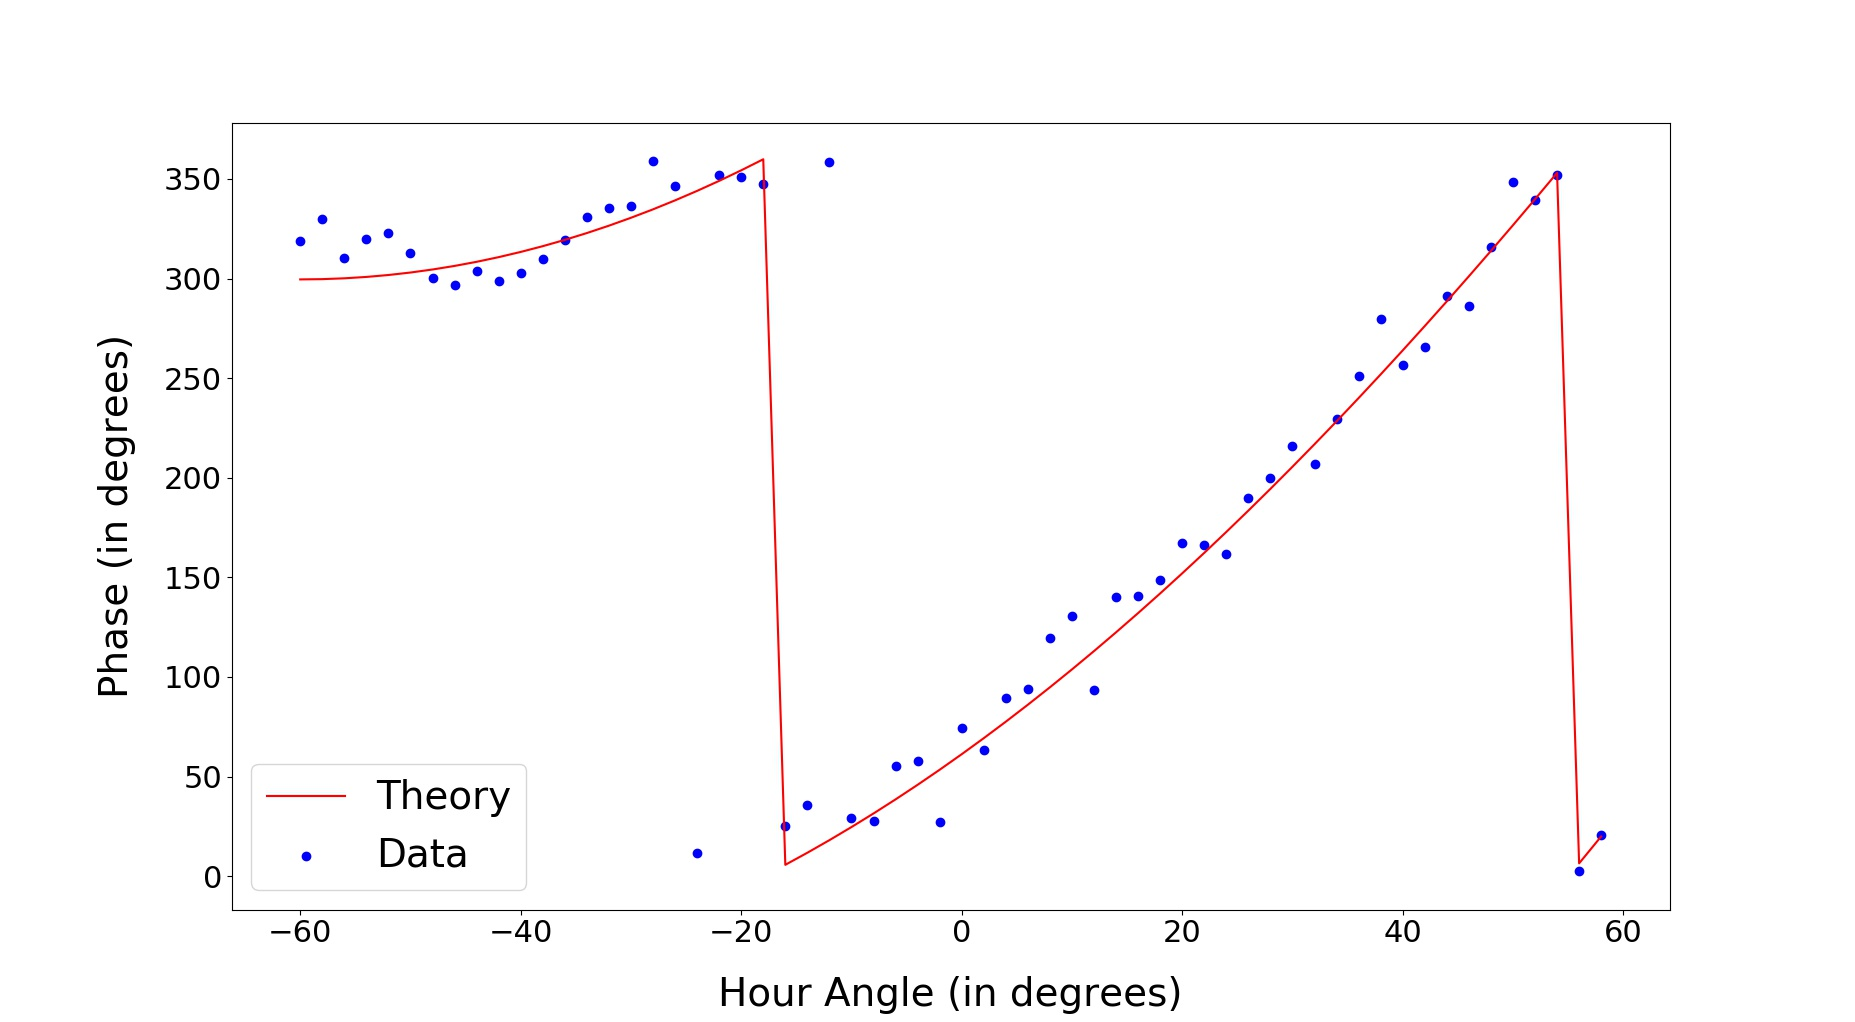
\includegraphics[scale=.25]{/home/matthew/Main/RadioAstronomy/Homework7/Even_Dec12.jpeg}
\caption{Pictured above is the even part of the data as compared to the even part of the theoretical values produced when a value of $\triangle$Bx= -.155 and $\triangle$ Bz= .659 is used.}
\end{figure}

The second step was to take the odd part of the data at 12.5$\degree$ declination and determine $\triangle$By using the same method as for $\triangle$Bx.

\begin{figure}[H]
\centering
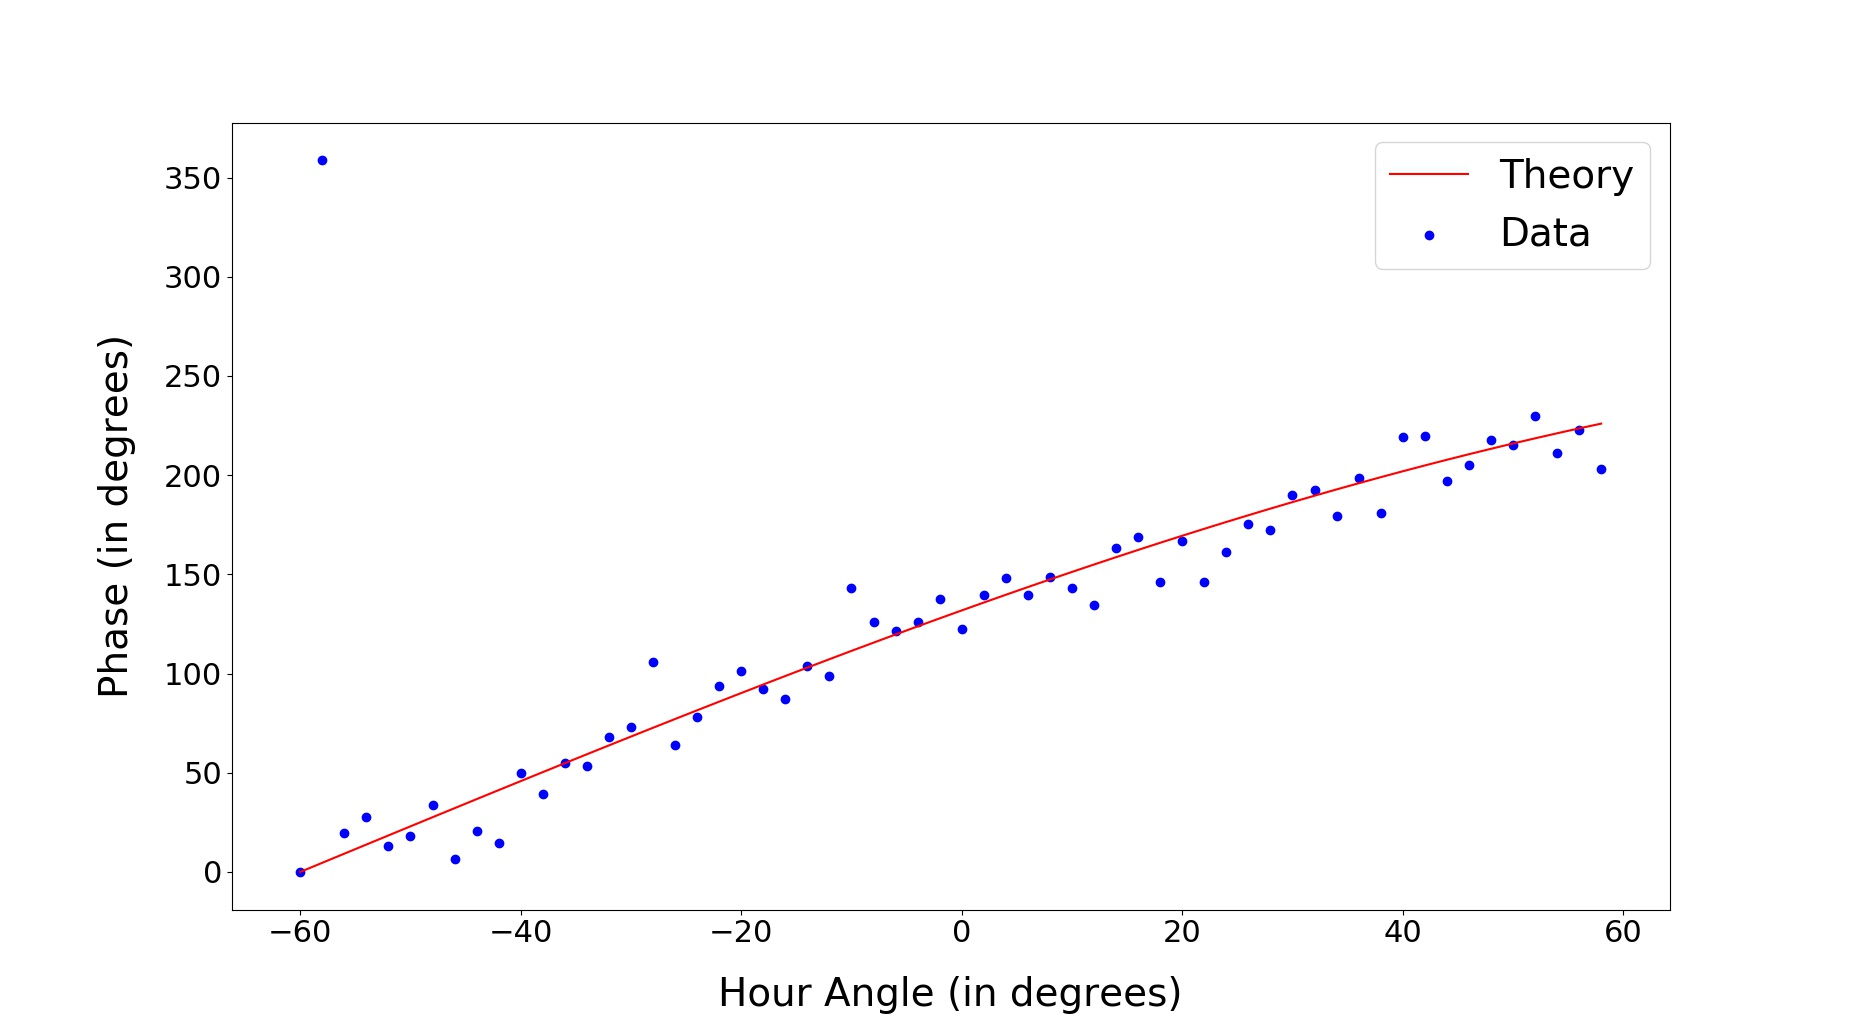
\includegraphics[scale=.25]{/home/matthew/Main/RadioAstronomy/Homework7/Odd_Dec12.jpeg}
\caption{Pictured above is the odd part of the data as compared to the odd part of the theoretical values produced when a value of $\triangle$By = -.045 is used. $\triangle$Bz does not affect the odd part of the data.}
\end{figure}

Then, for the 12.5$\degree$ declination data, we have the match that has been plotted below.  

\begin{figure}[H]
\centering
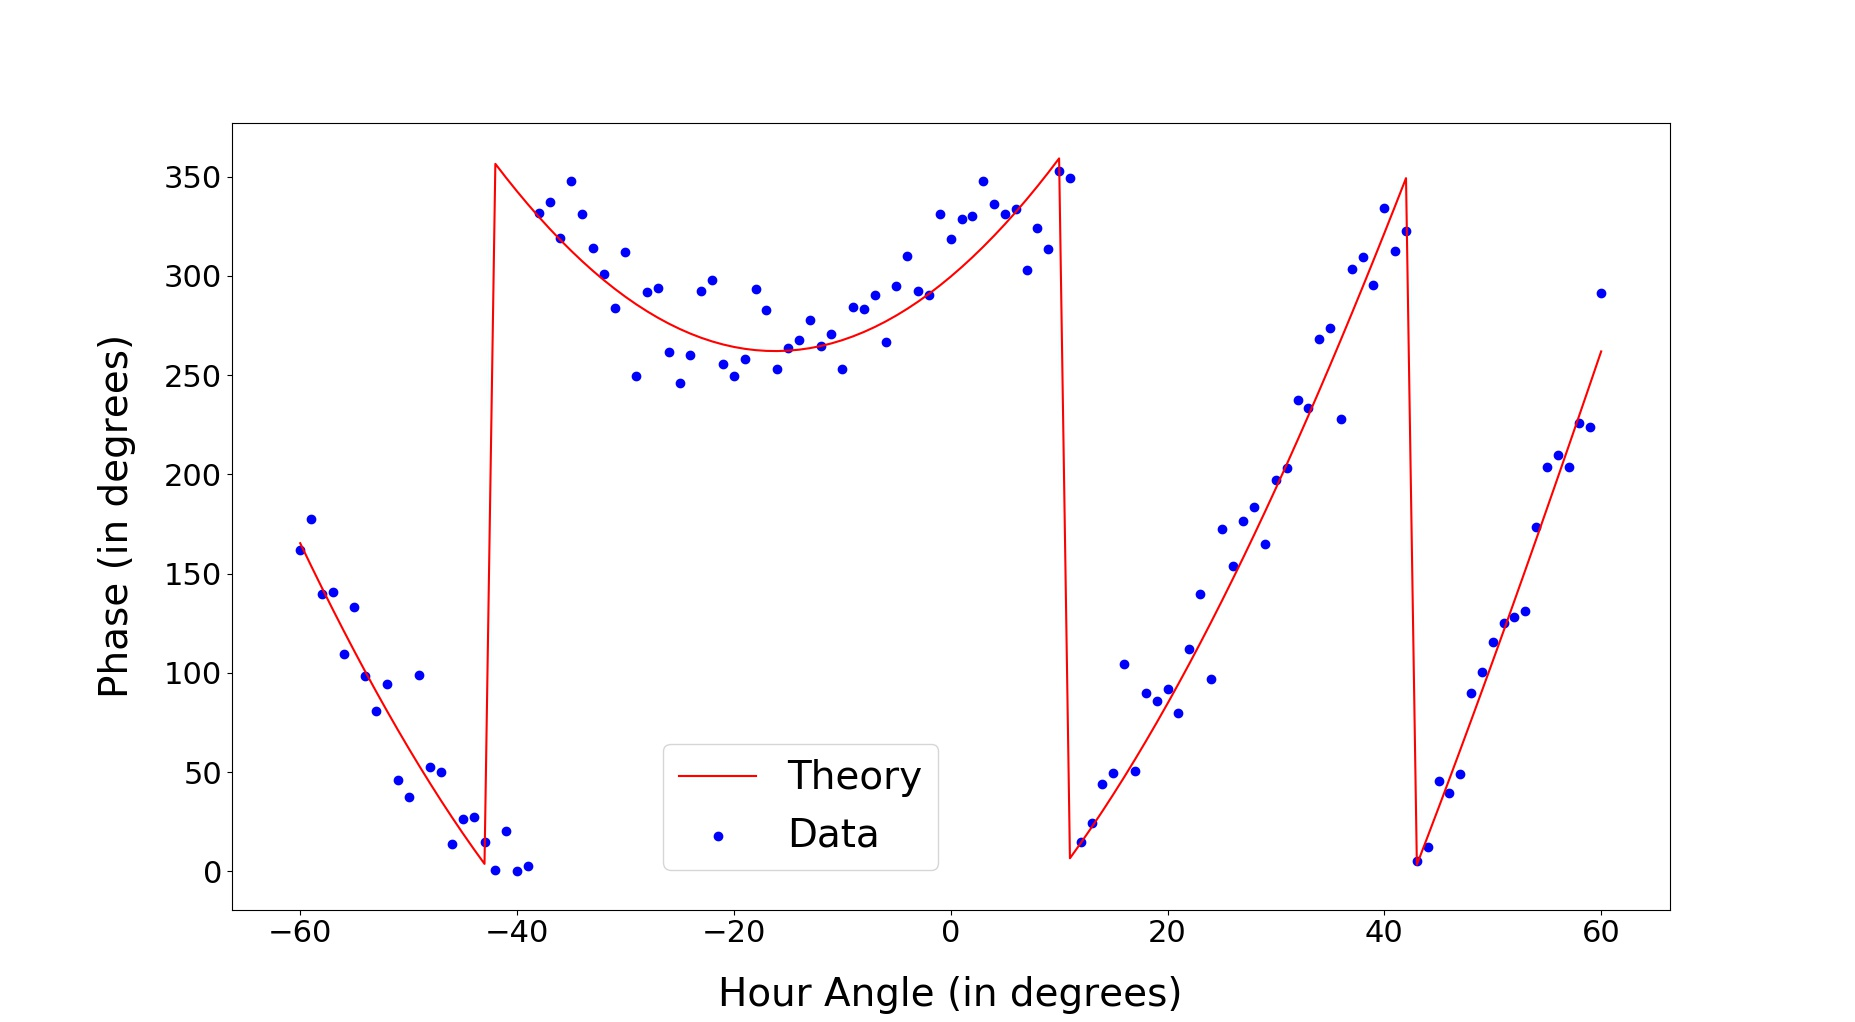
\includegraphics[scale=.25]{/home/matthew/Main/RadioAstronomy/Homework7/Total_Dec12.jpeg}
\caption{Pictured above is the 12.5$\degree$ declination data as compared to the theory when a value of $\triangle$Bx= -.155, $\triangle$By= -.045, $\triangle$Bz= .659 is used.}
\end{figure}

Now, of course, we must determine $\triangle$Bz, which was significantly more challenging than I had anticipated, and I found multiple minimums which can satisfy this, which I will explain.  If we take the current values and plot them against the 33.2$\degree$ declination data, we of course do not get a match.  Since $\triangle$Bz is related to the phase offset, there are periodic values which satisfy either the 12.5$\degree$ declination or 33.2$\degree$ declination individually.  The goal is to find one which matches both of them to within a reasonable error.

This process began by assuming that the $\triangle$Bx and $\triangle$By determined by the above process are correct for both declinations.  Then, I created an array of possible $\triangle$Bz values ranging from [-2,2].  I set this limit because there were several other possible values for $\triangle$Bz in the [-10,10] range, so I assumed that $\triangle$Bz had to be less than two.  A third, lower declination value would remove this ambiguity.  
If we plot the least squares values for both declinations for this range of $\triangle$Bz values, we get the plot shown below.

\begin{figure}[H]
\centering
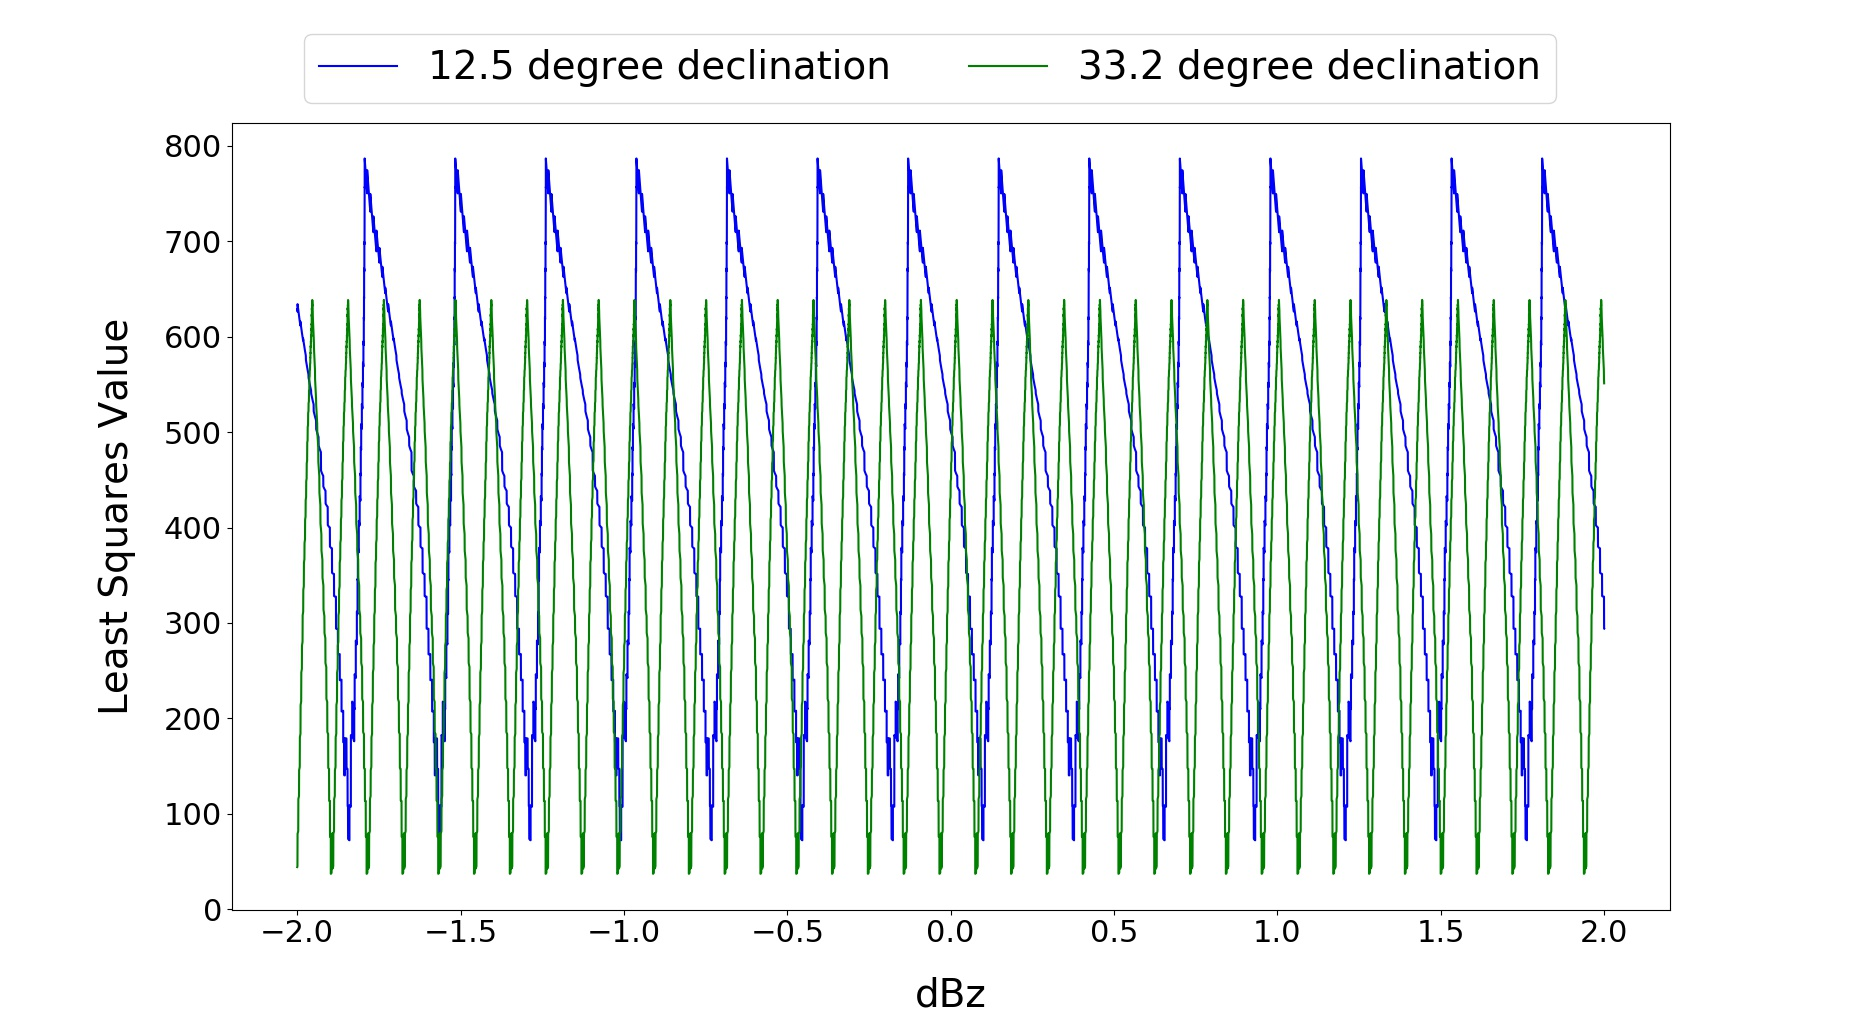
\includegraphics[scale=.25]{/home/matthew/Main/RadioAstronomy/Homework7/LstqrCompare.jpeg}
\caption{Pictured above is the least squares comparison between the 12.5$\degree$ and 33.2$\degree$ declination data when values of $\triangle$Bx = -.155 and $\triangle$By = -.045 are used.  As can be seen, the minimum least squares values match up as specific values of $\triangle$Bz.}
\end{figure}

The best match found within this range was at $\triangle$Bz = -1.565, which is plotted below in a zoomed window of Figure 4.

\begin{figure}[H]
\centering
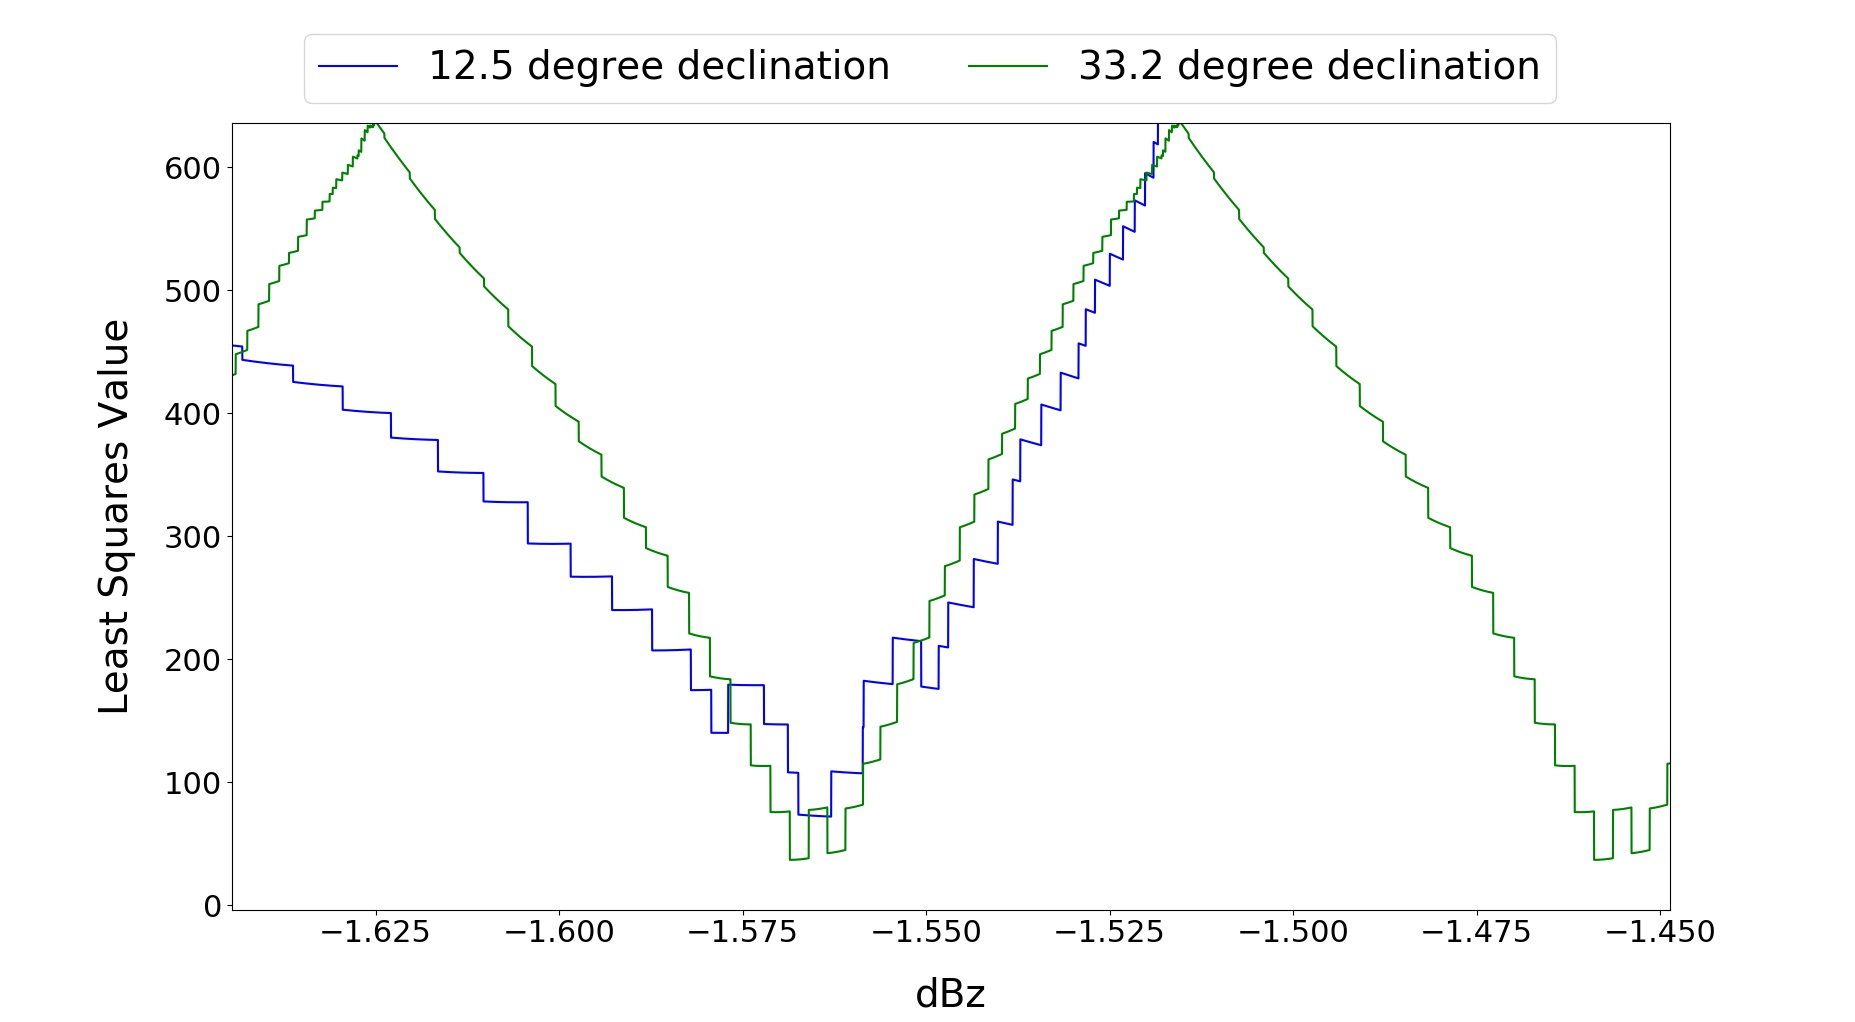
\includegraphics[scale=.25]{/home/matthew/Main/RadioAstronomy/Homework7/LstqrCompareZoom.jpeg}
\caption{Pictured above is a zoomed in window of Figure 4, about the location where the most likely $\triangle$Bz is located.  Others values were close, but this one showed the best match between the two data sets.}
\end{figure}

From this analysis, it was determined that $\triangle$Bz = -1.565.  It should be noted that a small error in $\triangle$Bx could significantly alter this result, but I couldn't get my shuffling program to work correctly in order to search around $\triangle$Bx values when a $\triangle$Bz had been selected.

\begin{figure}[H]
\centering
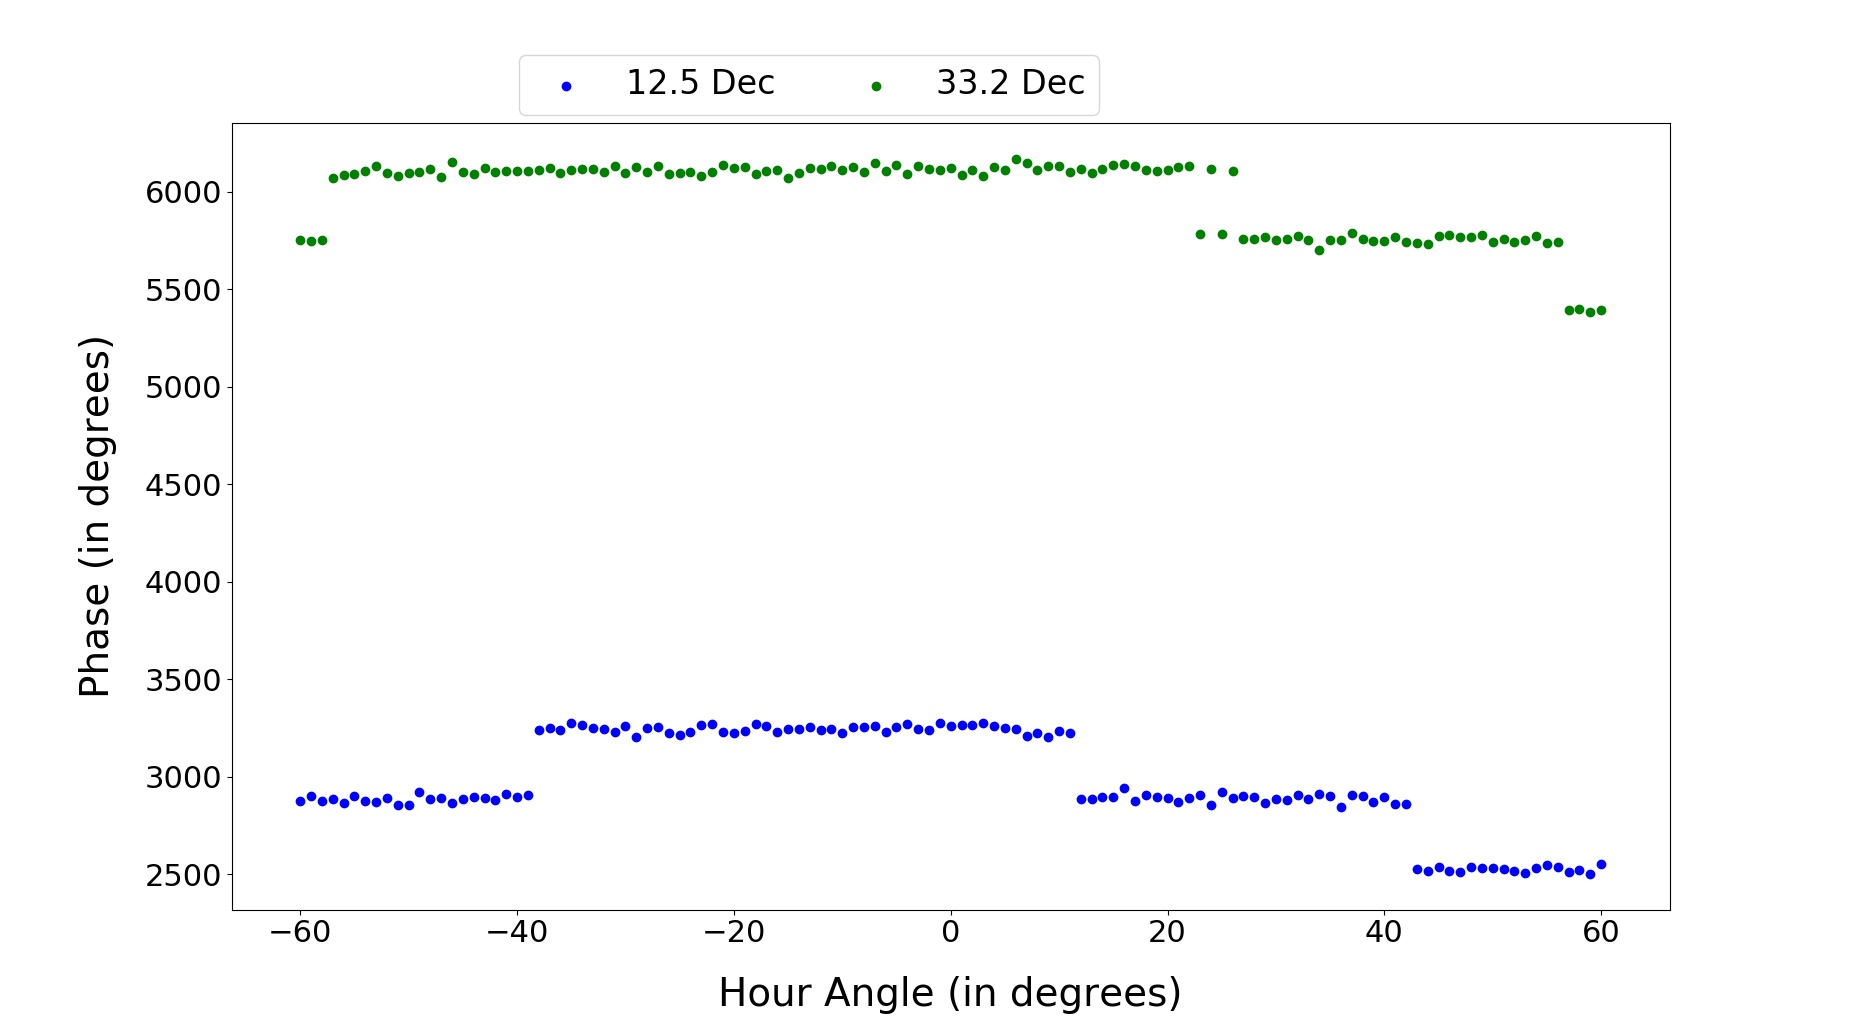
\includegraphics[scale=.25]{/home/matthew/Main/RadioAstronomy/Homework7/DataNoTheoryNoMod.jpeg}
\caption{Pictured above is the data with the theory removed, but this data has not been subjected to a modulo function, as the data in the first plot was.}
\end{figure}
\end{document}